\chapter{相关技术与工作}

\section{传统视频编辑方法}

早期的肖像视频编辑主要依赖于生成对抗网络(GAN),StyleGAN2\cite{karras2020analyzing}在图像生成方面取得成功后,许多工作者
开始将预训练的GAN模型应用于肖像编辑,例如3D-FM GAN\cite{liu20223d}引入StyleGAN以在保留人脸特征的同时实现3D人脸编辑;
此外,也有工作将其应用于肖像的风格化,DualStyleGAN\cite{yang2022pastiche}针对当时即便使用大量同类训练数据也只能实现单一风格化的问题,
引入StyleGAN实现了利用一张模板的风格化肖像生成。但是由于StyleGAN2的表示能力有限,这些工作难以稳定地
在复杂场景下实现高质量的肖像生成。

为了寻求更强的表示能力,研究者们尝试使用3D表示来进行肖像编辑。ClipFace\cite{aneja2023clipface}引入了三维网格来表示人脸,用自监督的生成模型
来实现人脸的编辑与动画。然而受限于三维网格的表示能力,这些工作存在身份失真与动作失真等问题。NeRF\cite{mildenhall2021nerf}在三维重建方面
取得巨大突破后,许多工作\cite{abdal20233davatargan}\cite{bao2024geneavatar}\cite{sun2023next3d}也引入NeRF进行肖像编辑,但这些工作仍然不能满足许多应用的需要。

扩散模型被提出并获得巨大成功后,许多工作尝试利用扩散模型强大的生成能力。Arc2Face\cite{papantoniou2024arc2face}等工作在2D肖像图片的生成与
编辑方面取得了进展;在3D方面,扩散模型被应用于文字提示下的3D人脸生成\cite{han2023headsculpt}\cite{zhang2023dreamface},
而Avatarstudio\cite{mendiratta2023avatarstudio}和Control4D\cite{shao2024control4d}则尝试将扩散模型应用于3D人脸编辑,
但它们都需要多角度的动态视频序列作为输入来建模3D人脸,这在现实中比较难以获取。

\section{PortraitGen技术原理}

PortraitGen作为当前先进的肖像视频编辑技术,其核心创新点体现在以下三个关键方面。

\subsection{3D高斯场表示}

\subsubsection{3D高斯场景表示}
在PortraitGen中,我们将视频编辑任务从2D提升至3D,并采用3D高斯溅射\cite{kerbl20233d}来表示场景。具体而言,
我们用数百万个3D高斯椭球来表示场景,对于每个以$\symbf{x}_0$为球心的高斯分布,我们有
\begin{equation}
    g(\symbf{x})=\exp{-\frac{1}{2}(\symbf{x}-\symbf{x}_0)^T\symbf{\Sigma}(\symbf{x}-\symbf{x}_0)}
\end{equation}
其中$\symbf{\Sigma}$为协方差矩阵,通过旋转和缩放控制椭球的形状,有分解
\begin{equation}
    \symbf{\Sigma}=\symbf{R}\symbf{\Lambda}\symbf{\Lambda}^T\symbf{R}^T
    \label{cov-decom}
\end{equation}
其中$\symbf{R}$为旋转矩阵,$\symbf{\Lambda}$为缩放矩阵。为了将三维的场景映射到二维平面,
我们还需要定义每个3D高斯的不透明度$\alpha$和球谐函数系数$\symbf{h}$,以控制光照和颜色信息。因此,我们可以将
一个3D高斯表示为$\{\symbf{x}_0,\symbf{q},\symbf{s},\alpha,\symbf{h} \}$,其中$\symbf{q}$与$\symbf{s}$为
旋转变换对应的四元数和缩放变换对应的向量。

\subsubsection{参数优化}
3D高斯场采用了可微分的溅射渲染,通过将3D高斯投影到2D屏幕空间,我们可以计算每个像素的颜色
\begin{equation}
    C(\symbf{p})=\sum_{i\in N}c_i\alpha_i\prod_{j=1}^{i-1}(1-\alpha_j)
\end{equation}
其中$c_i$为第$i$个高斯的颜色,基于视角可以由球谐函数决定。为了优化由稀疏点云重建的3D高斯场,
我们将给定视角下的渲染结果与真实结果进行比对,定义损失函数为
\begin{equation}
    \mathcal{L}=(1-\lambda)\mathcal{L}_1+\lambda\mathcal{L}_\text{D\_SSIM}
\end{equation}
其中$\mathcal{L}_1$为渲染的像素差异,描述了渲染结果与真是结果的光度差异;$\mathcal{L}_\text{D\_SSIM}$
为基于感知的损失函数,用于衡量图像的结构相似性。我们选用随机梯度下降(SGD)来优化3D高斯的参数,
包括高斯的位置、协方差、不透明度和颜色。注意到协方差矩阵$\symbf{\Sigma}$有其物理意义,只有半正定矩阵
是合理的,但是SGD优化难以添加约束条件,因此考虑到协方差矩阵的分解形式~\eqref{cov-decom},我们转而对
代表缩放的向量$\symbf{s}$与代表旋转的四元数$\symbf{q}$进行优化。

初始的3D高斯直接由点云重建,而这种2D到3D的映射往往无法满足精细表示的需要,因此我们的优化也需要
有3D高斯的自适应操作,包括:
\begin{enumerate}
    \item \textbf{删除}:当3D高斯的透明度小于阈值$\epsilon_{\alpha}$时,说明此时3D高斯对场景表示的贡献较小,可以删除;
    \item \textbf{密集}:区域没有被3D高斯覆盖与过度覆盖都说明当前重建不够,需要修改目前的3D高斯,以更好地表示场景:
        \begin{itemize}
            \item 当区域没有被3D高斯完全覆盖时,将已有的3D高斯复制并按照梯度方向移动到空白位置;
            \item 当区域被3D高斯过度覆盖时,将大3D高斯按照$\phi=1.6$的比例分成两个小的3D高斯;
        \end{itemize}
    \item \textbf{特殊处理}:与其他体积表征的方法类似,在相机附近可能有悬浮3D高斯导致优化停滞,因此需要每迭代3000轮后将这些3D高斯的透明度$\alpha$设置为接近0。
\end{enumerate}

\begin{figure}[ht]
    \centering
    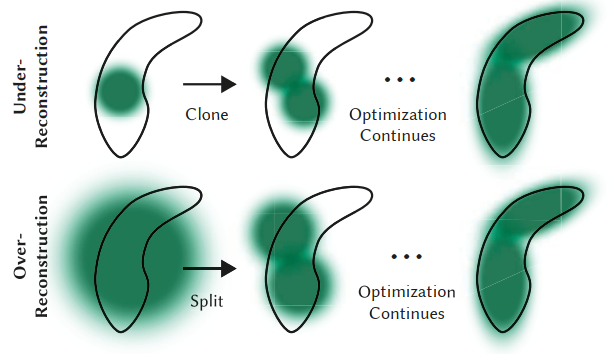
\includegraphics[width=0.5\textwidth]{source/img/gauss_recon.png}
    \caption{3D高斯的密集}
\end{figure}

\subsubsection{可微光栅化渲染}

3D高斯的光栅化过程主要分为四个步骤:
\begin{enumerate}
    \item \textbf{分块}:将屏幕空间划分为$16\times 16$的小块,对每个小块保留与视锥相交超过99\%的高斯球;
    \item \textbf{排序}:为每个高斯分配一个键,携带视图空间深度与块ID信息,并利用GPU基数排序,为每个块生成一个高斯列表;
    \item \textbf{光栅化}:每个块启动一个线程块,协作加载高斯到共享内存。对每个像素,从前到后遍历列表,累积颜色和$\alpha$值,当像素的$\alpha$值达到饱和(接近1)时,停止处理;
    \item \textbf{反向传播}:在反向传播时,重新遍历排序后的高斯列表,但方向是从后到前。这样可以在计算梯度时恢复中间的$\alpha$值,无需存储中间结果增加内存消耗。
\end{enumerate}

\subsection{神经高斯纹理机制}

在标准的3D高斯溅射中,每个3D高斯的颜色通过球谐函数的系数来表示,而这种表示存在一些问题:一方面,球谐系数仅能建模低频的光照变化,难以表现高频的细节,如笔触、艺术风格等;另一方面,
强制使所有视角严格遵守物理光照,阻碍了3D高斯在会真实感渲染方面的应用,例如卡通风格的轮廓线等。PortraitGen用可学习的特征来代替每个3D高斯的球谐函数,实现了更强的表达能力。

我们使用SMPL-X\cite{pavlakos2019expressive}作为人体模型的表示方法,SMPL-X的定义为
\begin{align}
    M(\beta,\theta,\psi)&=W(T_p(\beta,\theta,\psi), J(\beta),\theta, \mathcal{W})\\
    T_p(\beta,\theta,\psi)&=\bar{T}+B_S(\beta;\mathcal{S})+B_E(\psi;\mathcal{E})+B_P(\theta;\mathcal{P})
\end{align}
其中$\beta$、$\theta$、$\psi$分别为形状、姿态与表情参数;$W$为线性混合蒙皮函数,$J$为稀疏线性回归器,可以从输入网格顶点回归出三维关节位置,$\mathcal{W}$
为混合权重,在旋转时起平滑作用。

我们在SMPL-X模型的UV表面绑定3D高斯场$\phi$,通过纹理坐标$(u,v)$来索引特征,这样在网格动态变形时高斯能随之运动从而保持拓扑的一致性。利用UV空间的参数映射$\mathcal{G}$,我们可以得到某一帧的3D高斯场
\begin{equation}
    (\symbf{X}_0,Q,S,O,F)=\mathcal{F}(M(\beta,\theta,\psi),\mathcal{G},\phi)
\end{equation}

\subsection{表情相似性引导与感知编辑}

在PortraitGen的编辑过程中,需要迭代编辑视频数据集,而在反复编辑视频帧的过程中,每次编辑都可能引入微小表情偏差,多次迭代后偏差放大,
导致面部表情和个性化特征会逐渐退化,如笑容僵硬、五官变形等。为了解决这一问题,我们采用3D表情识别模型EMOCA\cite{danvevcek2022emoca}提取表情潜码
\begin{equation}
    z_{\text{exp}}=E_{\text{EMOCA}}(I) \in \mathbb{R} ^{50}
\end{equation}
并通过$L2$损失约束编辑后的表情特征
\begin{equation}
    \mathcal{L}_{\text{exp}}=||E_{\text{EMOCA}}(I_{\text{edit}})-E_{\text{EMOCA}}(I_{\text{src}})||_2^2
\end{equation}
实现了仅约束表情肌肉运动而不限制外观风格变化。

\section{系统开发技术}

考虑到编辑算法的特性、部署环境的软硬件支持以及提供服务的具体场景,我们在系统开发过程中采用了以下工具作为技术栈。

\subsection{Next.js}

Next.js是一个基于React的现代前端开发框架\cite{lazuardy2022modern},它支持同时存在构建时预渲染页面(SSG)和请求时渲染页面(SSR)的混合模式,
并且支持增量静态生成,从而可以实现用户访问页面时即时加载构建时生成的静态HTML文件,大大提升用户体验。在开发过程中,
它支持TypeScript,开发者可以获取静态类型检查,增强代码的健壮性;此外,它具备快速刷新的功能,给予开发者快速、
可靠的实时编辑体验,并已经在Facebook级别的应用上规模上得到验证。

Next.js开发中,我们还使用了React 16.8中引入的Hook函数\cite{reacthooks2019}\cite{bugl2019learn},可以在不编写类的情况下在函数组件中使用状态和其他React特性。
具体来说,在 React 16.8 之前,函数组件被称为"无状态组件",因为它们无法管理自身的状态或使用生命周期方法。
Hook 的出现彻底改变了这一局面,使函数组件能够拥有类组件的所有能力(见表~\ref{tab:hooks})。
例如我们使用useState来管理函数中的状态,它返回一个状态变量和更新该状态的函数,
状态更新将触发组件的重新渲染;我们使用useEffect来实现多个生命周期方法的功能,当依赖数组发生变化时执行副作用函数,
并通过返回函数来清理副作用。Hook特性可以提取组件逻辑并在多个组件间共享,同时解决了高阶组件与渲染属性带来的多层嵌套问题。

\begin{table}
    \centering
    \caption{Hook与类组件的对比}
    \label{tab:hooks}
    \begin{tabular}{cll}
        \toprule
        特性   & 类组件  &Hook                                  \\
        \midrule
        状态管理 & this.state / setState & useState/useReducer \\
        生命周期 & 多个独立方法 & useEffect统一处理   \\
        代码组织 & 分散为多个方法 & 相关逻辑集中  \\
        \bottomrule
    \end{tabular}
\end{table}

\subsection{Flask}

Flask \cite{flask}是一个轻量级的 Python Web 框架,被称为"微框架"(microframework),因为它核心简单但可通过扩展添加功能。
基于以下的开发需求,我们选择Flask作为后端框架:
\begin{enumerate}
    \item \textbf{轻量级}:作为轻量级Web框架,Flask不强制使用任何特定库,可以根据需求灵活扩展;
    \item \textbf{RESTful API}:Flask采用Werkzeug路由引擎,支持动态URL规则,方便定义API节点,适合开发RESTful API;
    \item \textbf{异步任务处理支持}:Flask支持Redis作为任务队列,方便处理异步任务;
    \item \textbf{算法适配}:使用python开发使其与各种AI算法适配,方便调用处理算法与后续算法扩展。
\end{enumerate}

\subsection{数据管理技术}

本系统采用MySQL作为数据库,主要基于以下考量:
\begin{enumerate}
    \item \textbf{事务支持}:MySQL保证事务的原子性、一致性、隔离性和持久性,适合处理复杂的数据操作;
    \item \textbf{SQL查询性能}:MySQL的SQL查询性能优秀,足以满足系统的数据库操作要求;
    \item \textbf{关系型数据库}:MySQL是一种关系型数据库,适合存储结构化数据,如用户信息、视频信息、请求信息等。
\end{enumerate}

另外我们使用Redis\cite{redis}管理任务队列,作为高性能的键值对存储数据库,适合存储任务信息,如任务ID、任务状态、任务进度等,并且
由于其支持发布/订阅模式,方便实现任务队列的异步处理。